\documentclass{article}
\usepackage{graphicx}

\title{Balloons Project - System Architecture}
\author{Andrew Dodd}
\begin{document}
\maketitle

\section{Introduction}
This document gives an overview of the entire Balloons Project system along 
with a brief description of its main components. Further details on each 
individual system can be found in the corresponding section of documentation.

\section{System Overview}

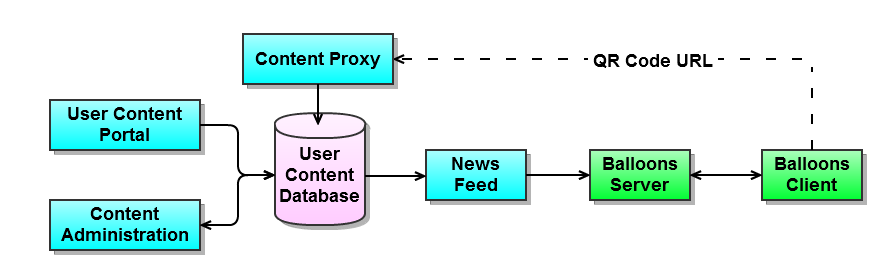
\includegraphics[width=\textwidth]{Diagrams/System-Architecture-Diagram.png}

Items in light blue are web-based components, written in PHP and producing 
either HTML/JS/CSS page output or JSON objects. Green items are written in C\#
4.0 and the pink database is an SQL RDBMS. The QR Code URL is accessed by users
when viewing content and is usually interpreted by a third-party device such as
a mobile phone.

\subsection{User Content Database}
The User Content Database is used to store user content submitted from the web
front end. Important information stored includes general content information 
such as title and image; when the content was submitted; and the name of the 
user who submitted the content (for moderation purposes and deter the 
submission of inappropriate content). The database also stores the current 
"score" of each custom article; this comes from the content voting system. 

\subsection{Web-Front Ends: User Content Portal \& Content Administration}
Two web-based front ends exist. The User Content Portal is used by users to 
submit custom content which will appear as a balloon on the system. Once 
content is submitted it is stored in the User Content Database. The Content
Administration section lets administrators review and moderate any user 
generated content and will be primarily used to remove offensive or otherwise
inappropriate content.

\subsection{Content Proxy}
The content proxy is used to provide an interface for end users to rate content
by either giving it an up or down vote. Once the vote is cast, it is stored
against the story in the database and the user is redirected to the URL of the
content.

\subsection{News Feed}
The News Feed component is responsible for choosing some content for the 
front-end; ratios for the different content-types are defined in the feed 
whilst the number of items to fetch is determined by the caller. When 
requested, it generates a JSON object which is consumed by the Balloons Server.

\subsection{Balloon Server}
The Balloon Server is responsible for coordinating all the balloons on the 
Balloon Clients. This involves parsing the News Feed to get balloons, sending
balloons to each client and dealing with balloons travelling between screens 
as well as balloons being popped by the user. 

When a client connects to the server, it must generate new balloons; this 
causes the feed to be refreshed. Once the balloons are generated they are 
pushed to the new client. If a client disconnects, all its balloons are 
randomly redistributed to the other screens.

\subsection{Balloon Client}
The Balloon Client displays balloons in a graphical manner and allows users to
interact with the display. The main elements of the display are the balloons 
themselves which have a short description of the article they represent and the
news-reader element which displays the full content of the article as well as
an image and QR Code which directs users via the Content Proxy to the news item.

\end{document}